\begin{figure*}[t]
    \center
    \jsubfig{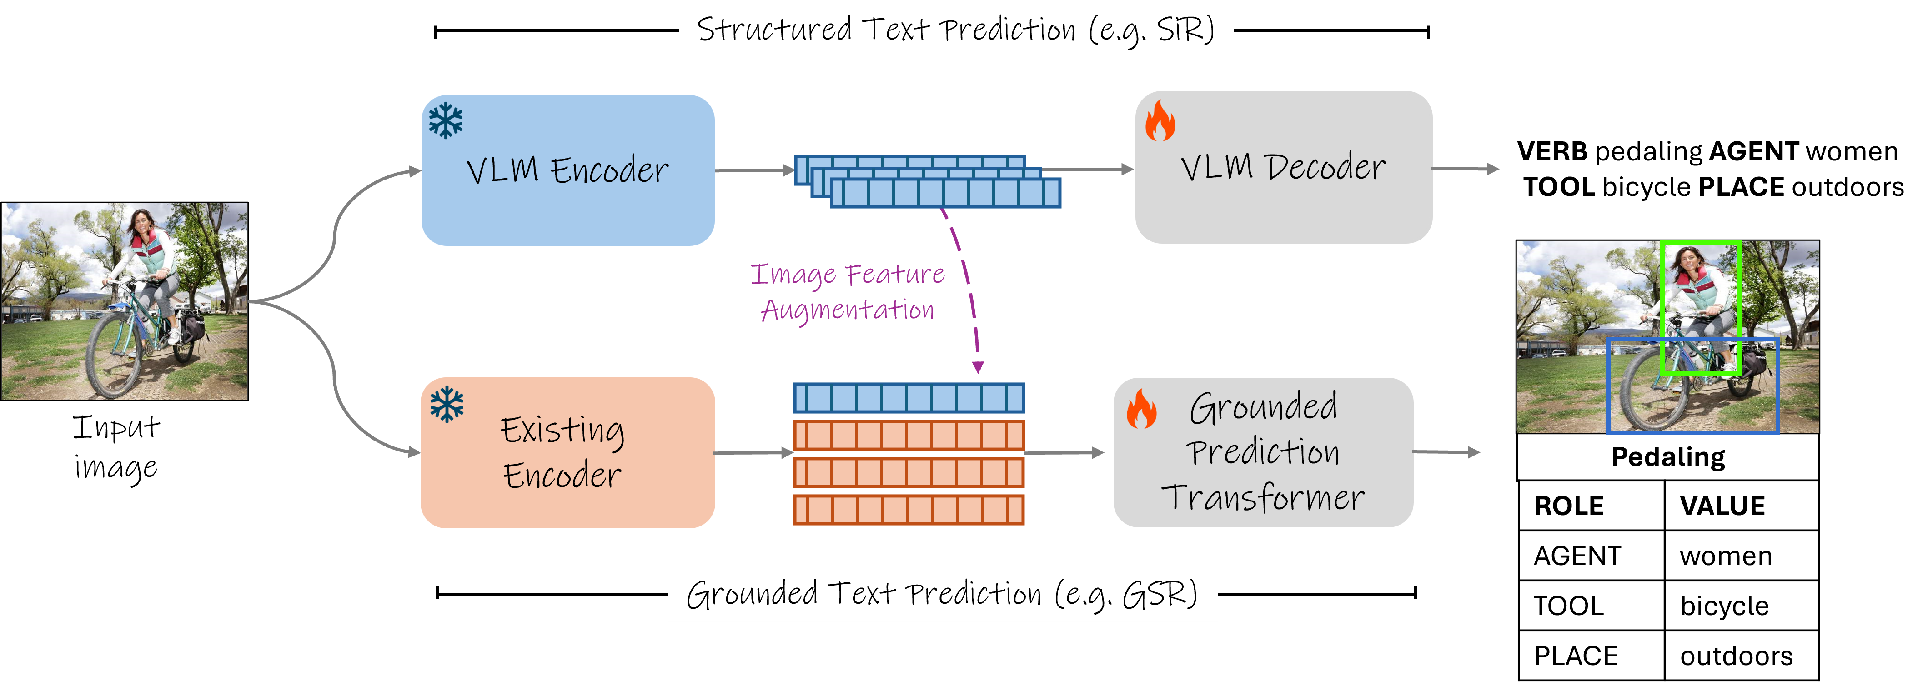
\includegraphics[width=1\textwidth]{figures/system/method_13_11.pdf}
    }   
    
    \caption{\textbf{Our framework.} We illustrate our framework for performing high-level (top) and grounded (bottom) tasks, exemplified by the tasks of \sr and GSR in the figure. For overall scene understanding tasks we add trainable weights to the VLM text decoder and fine-tune these using a standard token-wise language modeling objective to predict the desired labels as formatted text. For grounded prediction tasks we concatenate the V\&L embeddings to the existing vision backbone embeddings. The existing model is trained according to its initial formulation.}
    \label{fig:system}
    
\end{figure*}
